%!TEX root = ../main.tex

\chapter{Einleitung}
\label{chap:einleitung}

Restaurants sind Orte, an denen Menschen nicht nur gutes Essen genießen, sondern auch eine Auszeit vom Alltag nehmen können. Ob für ein romantisches Dinner, ein schnelles Mittagessen oder ein entspanntes Treffen mit Freunden – die Gastronomie bietet für jeden Anlass das passende Ambiente. Doch in einer Welt, die immer schneller wird und in der Zeit oft zur kostbarsten Ressource wird, stehen auch Restaurants vor der Herausforderung, sich an die Bedürfnisse ihrer Gäste anzupassen.

Ein neues Konzept revolutioniert nun das Restauranterlebnis: Kunden können bereits beim Betreten des Restaurants oder bei der Reservierung angeben, wie viel Zeit sie für ihren Besuch einplanen. Ob 30 Minuten für eine schnelle Mahlzeit oder zwei Stunden für ein ausgedehntes Dinner – dieses innovative Modell ermöglicht es, den Service individuell auf die Wünsche der Gäste abzustimmen. So wird nicht nur die Effizienz gesteigert, sondern auch das Restauranterlebnis persönlicher und flexibler gestaltet.

In dieser Arbeit wird das Konzept der zeitbasierten Reservierung genauer untersucht und ein optimiertes intelligentes Mutliagentensystem vorgestellt, das die Umsetzung in einem Restaurant, der \emph{Cucina intelligente di Massimo}, unterstützt.

\begin{figure}[h]
    \centering
    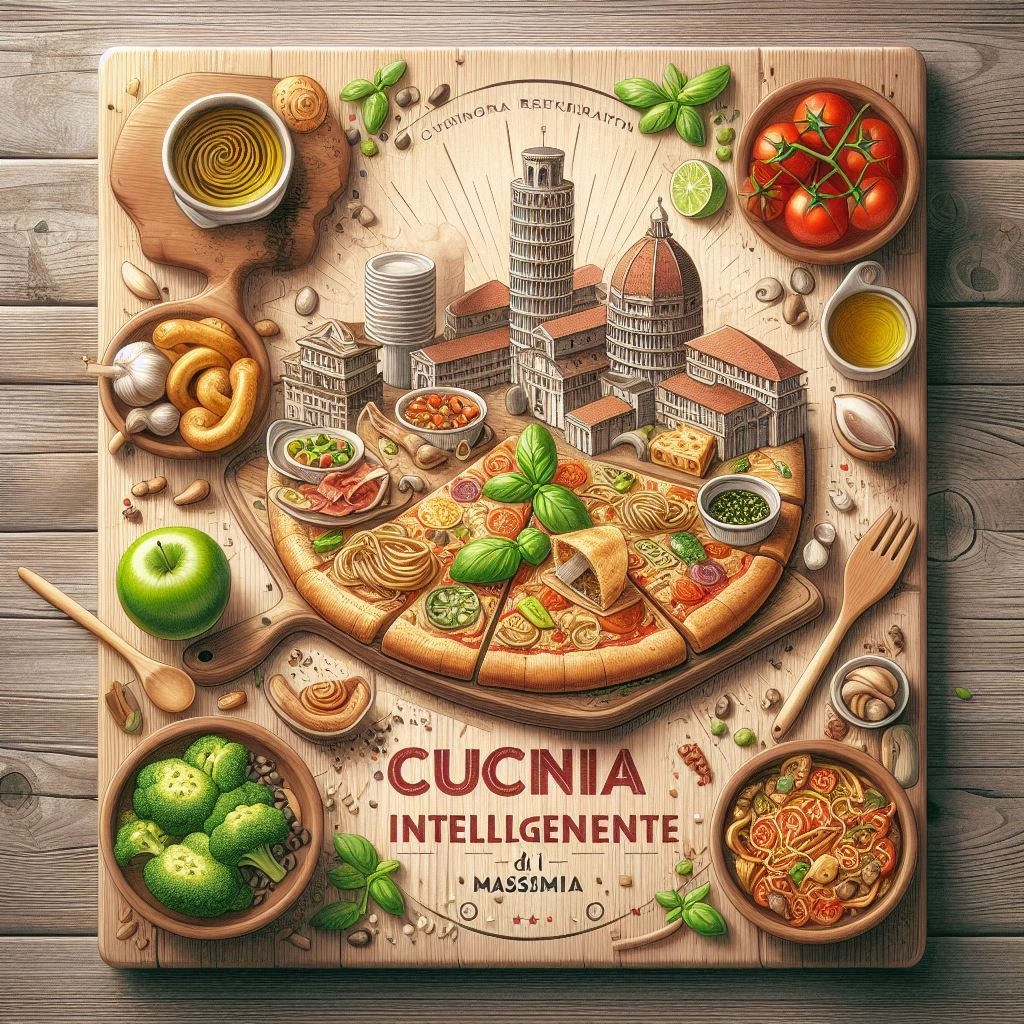
\includegraphics[width=0.5\textwidth]{img/cover.jpg}
    \caption{Cover}
    \label{fig:cover}
\end{figure}

% Im Folgenden werden die Anforderungen an das System analysiert, die Architektur und die Funktionsweise des Systems beschrieben und die Implementierung sowie die Evaluation des Systems vorgestellt. Abschließend werden die Ergebnisse zusammengefasst und ein Ausblick auf mögliche Erweiterungen gegeben.